\section{Case study: completely pivoted LU}

Linear algebra is ubiquitous in technical computing applications. At the same
time, the implementation of linear algebra libraries is generally considered a
difficult problem best left to the experts. A popular reference book for
numerical methods famously wrote, for example, that ``the solution of
eigensystems... is one of the few subjects covered in this book for which we do
\textit{not} recommend that you avoid canned routines''~\cite[Section 11.0, p.
461]{Press1992}. While much effort has been invested in making
numerical linear algebra libraries
fast~\cite{lapack,Gunnels2001,OpenBLAS,VanZee2013}, one nevertheless will
occasionally need an algorithm that is not implemented in a
standard linear algebra library.

One such nonstandard algorithm is the completely pivoted LU factorization. This
algorithm is not implemented in standard linear algebra libraries in
LAPACK~\cite{lapack}, as the conventional wisdom is the gains in numerical
stability in complete pivoting is not generally worth the extra effort over
other variants such as partial pivoting~\cite{Golub2013}.  Nevertheless, users
may want complete pivoting for comparison with other algorithms for a
particular use case.
%For example, one may be interested in comparing the
%results of an infinite dimensional LU factorization to its finite-dimensional
%approximation, in which case only the completely pivoted LU is defined in both
%cases~\cite{Townsend2014}.

In this section, we compare implementations and performance of this
algorithm in Julia with other high level languages that are commonly used for
technical computing: MATLAB, Octave, Python/NumPy, and R.
%Second, we
%rewrite the na\"ive Julia implementation for better performance, and
%demonstrate the effects of each transformation on execution time. We believe
%that this work flow reflects typical use cases of high level dynamic languages,
%where users first write na\"ive but verifiably correct implementations, then
%rewrite the implementation until sufficient performance can be achieved.



\subsection{Na\"ive textbook implementation}

Algorithm~\ref{alg:lucompletepiv} presents the textbook description of the LU
factorization with complete pivoting~\cite[Algorithm 3.4.3 (Outer Product LU
with Complete Pivoting), p. 132]{Golub2013}, and below it a direct translation
into a na\"ive Julia implementation. This algorithm is presented in MATLAB-like
pseudocode, and contains a mixture of scalar \lstinline|for| loops and
MATLAB-style vectorized indexing operations that describe various subarrays of
the input matrix $A$. Additionally, there is a description for the subproblem
of finding the next pivot at the start of the loop. Furthermore, the pseudocode
uses the $\leftrightarrow$ operation, denoting swaps of various rows and
columns of $A$. To translate the pivot finding subproblem into Julia, we used
the built-in \lstinline|indmax| function to find the linear index of the value
of the subarray \lstinline|A[k:n, k:n]| which has the largest magnitude, then
used the \lstinline|ind2sub| function to convert the linear index to a tuple
index. The $\leftrightarrow$ operator was implemented using vectorized indexing
operations, as is standard practice in high level languages like MATLAB.



\begin{algorithm}

\caption{Top: Textbook pseudocode describing the $LU$ factorization with
complete pivoting~\cite[Algorithm 3.4.3 (Outer Product LU with Complete
Pivoting), p. 132]{Golub2013}. The matrix $A$ is overwritten in-place with the
$LU$ factors, with $rowpiv$ and $colpiv$ containing the row and column pivots
respectively.
Bottom: An implementation of $LU$ factorization with complete pivoting in Julia,
which returns the result as a tuple. The ! at the end of the function name is
convention for a function with side effects (in this case, mutating $A$).
Unicode characters such as Greek letters and the $\ne$ operator are allowed in
Julia code, allowing for close notational correspondence with the textbook
description of the algorithm.}
\label{alg:lucompletepiv}

\begin{algorithmic}
\For {$k = 1:n - 1$}

    Determine $\mu, \lambda$ where $k \le \mu \le n$,  $k \le \lambda \le n$, so

    $\quad\left|A(\mu, \lambda)\right| = \max\{ \left|A(i, j)\right| : i=k:n, j=k:n \}$

    $rowpiv(k) = \mu$

    $A(k, 1:n) \leftrightarrow A(\mu, 1:n)$

    $colpiv(k) = \lambda$

    $A(1:n, k) \leftrightarrow A(1:n, \lambda)$

    \If{$A(k,k) \ne 0$}

        $\rho = k+1:n$

        $A(\rho, k) = A(\rho, k)/A(k, k)$

        $A(\rho, \rho) = A(\rho, \rho) - A(\rho, k) A(k, \rho)$
    \EndIf
\EndFor
\end{algorithmic}

\hrulefill

\begin{lstlisting}
function lucompletepiv!(A)
	n=size(A, 1)
	rowpiv=zeros(Int, n-1)
	colpiv=zeros(Int, n-1)
	for k=1:n-1
		Asub = abs(A[k:n, k:n]) #Search for next pivot
		$\mu$, $\lambda$ = ind2sub(size(Asub), indmax(Asub))
		$\mu$ += k-1; $\lambda$ += k-1
		rowpiv[k] = $\mu$
		A[[k, $\mu$], 1:n] = A[[$\mu$, k], 1:n]
		colpiv[k] = $\lambda$
		A[1:n, [k, $\lambda$]] = A[1:n, [$\lambda$, k]]
		if A[k,k] $\ne$ 0
			$\rho$ = k+1:n
			A[$\rho$, k] = A[$\rho$, k]/A[k, k]
			A[$\rho$, $\rho$] = A[$\rho$, $\rho$] - A[$\rho$, k] * A[k, $\rho$]
		end
	end
	return (A, rowpiv, colpiv)
end
\end{lstlisting}

\end{algorithm}

For comparison purposes, we also wrote na\"ive implementations in other high
level dynamics languages which are popular for technical computing. Here, we
considered MATLAB~\cite{matlab}, Octave~\cite{octave},
Python~\cite{python}/NumPy~\cite{numpy}, and R~\cite{rlang} (whose codes are
available in the Appendix). The codes were executed on a late 2013 MacBook Pro
running OS X
Yosemite 10.10.2, with Julia 0.4-dev+3970, MATLAB R2014b, Octave 3.8.1, Python
3.4.3 with NumPy 1.9.2 from the Anaconda 2.1.0 distribution, and R 3.1.3. Where
possible, we also tried to run variants with and without JIT compilation. In
MATLAB, the JIT compiler is on by default, but can be turned off with the
command \lstinline|feature accel off|. Octave's JIT compiler is experimental
and off by default, but can be enable with a command line switch. R provides a
JIT compiler in the \lstinline|compiler| library package. We do not have
JIT-compiled results for Python, as at this time of writing, neither PyPy
2.5.0~\cite{Bolz2009} nor Numba 0.17.0 was able to compile the code.\footnote{
The specialized fork of NumPy required to run on PyPy 2.5.0 did not build
successfully on neither Python 2.7.9 nor 3.4.3 on OSX. Numba 0.17.0, with the
\lstinline|@jit(nopython=True)| decorator, threw a
\lstinline|NotImplementedError| exception.}
The results are summarized in Figure~\ref{fig:scaling}, which shows the
near-perfect $O(n^3)$ scaling of the algorithm in each implementation, as well
as in Figure~\ref{fig:naivelangs}, which shows the execution times across the
different languages for a $1000 \times 1000$ matrix of \lstinline|Float64|s
with randomly sampled standard Gaussians.



\begin{figure}
	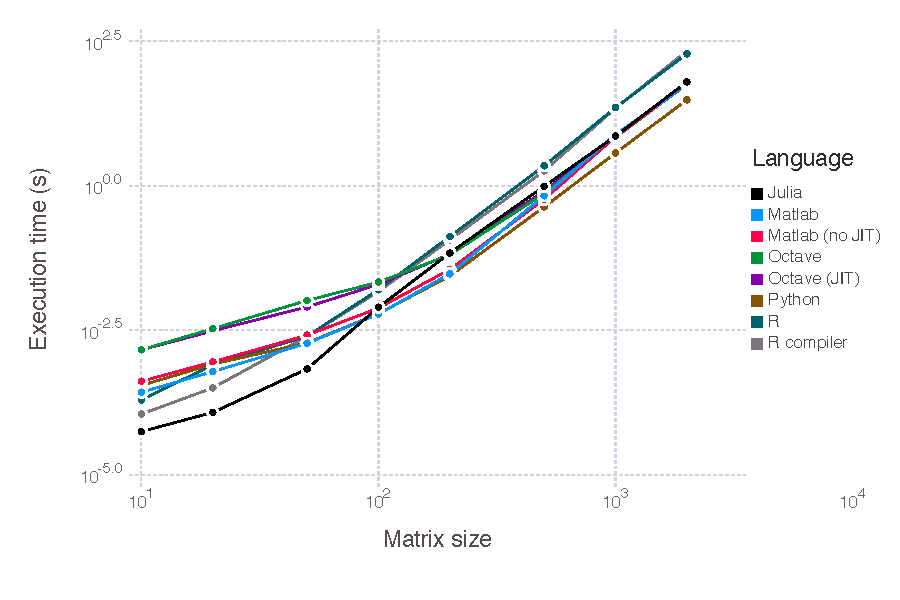
\includegraphics[width=\columnwidth]{data/fig-scaling}
	\caption{Scaling behavior of na\"ive implementations of the completely
	pivoted $LU$ algorithm on $N\times N$ random matrices in Julia, MATLAB,
	Octave, Python/NumPy, and R. By default, MATLAB's JIT compiler is on,
	whereas Octave's and R's are off. Julia code is listed in
	Algorithm~\ref{alg:lucompletepiv}.
	%, and the others are available in the
%Appendix. Plotted with \package{Gadfly.jl}.
}
	\label{fig:scaling}
\end{figure}

\begin{figure}
	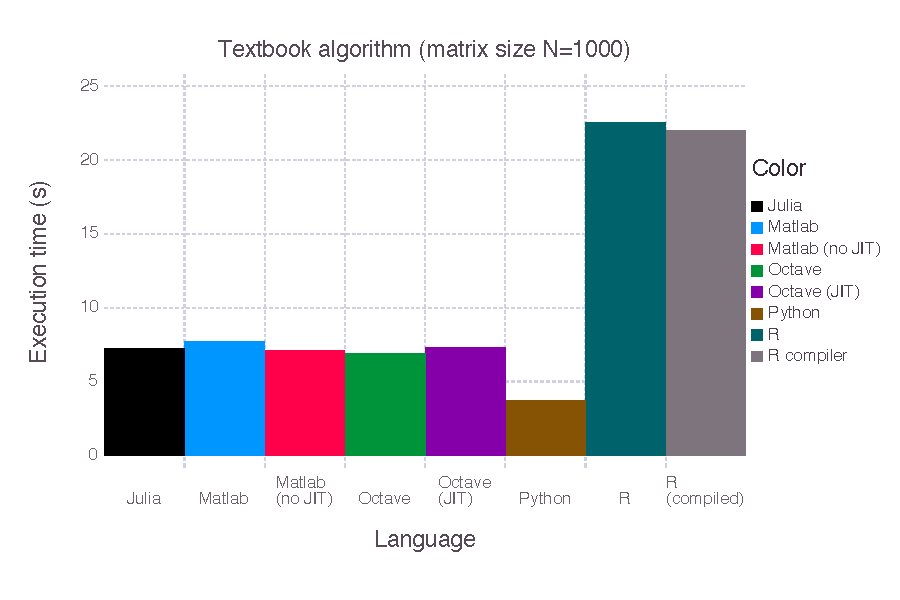
\includegraphics[width=\columnwidth]{data/fig-lang}
	\caption{Execution times of na\"ive implementations of the
	completely pivoted $LU$ algorithm on a $1000\times1000$ random matrix
	in Julia, MATLAB, Octave, Python/NumPy, and R. See Figure~\ref{fig:scaling}
	for further details.}
	\label{fig:naivelangs}
\end{figure}



\subsection{LU decomposition on arbitrary numeric types}

One major advantage to writing the $LU$ factorization code in pure Julia is
that \lstinline|lucompletepiv!| can run on any \lstinline|Matrix{T}|. So long
as the underlying element type \lstinline|T| is closed under the basic
arithmetic operations \lstinline|+|, \lstinline|-|, \lstinline|*|,
\lstinline|/|, \lstinline|abs|, and \lstinline|max|, the algorithm will run
just as it did on \lstinline|Float64| numbers. For example, one could compute
the completely pivoted $LU$ factorization on matrices of fixed point numbers
(provided by the \package{FixedPointNumbers.jl} package), or matrices of
rational numbers (built in \lstinline|Rational| types).

\begin{lstlisting}
using FixedPointNumbers

#Initialize 1000x1000 matrix of 32-bit fixed point 1s with 14 fractional bits
B = ones(Fixed32{14}, 1000, 1000)
lucompletepiv!(B)

#Initialize 1000x1000 matrix of unit rational numbers with 64-bit integer numerators and denominators fixed point 1s with 14 fractional bits
C = ones(Rational{Int64}, 1000, 1000)
lucompletepiv!(C)
\end{lstlisting}

Other interesting examples include the dual and hyperdual numbers provided by
the \package{DualNumbers.jl} and \package{HyperDualNumbers.jl} packages
respectively. Both types of numbers are used for forward mode automatic
differentiation, and can be used with \lstinline|lucompletepiv!| to take
derivatives of the $LU$ factorization itself. Computations over such arbitrary
numeric types would be difficult, if not impossible, in the other languages,
without reimplementing the basic algorithm \lstinline|lucompletepiv!| over and
over again.

While of course it is possible to build in more numeric types to the base
library of any programming language, the approach shown here is more general
by virtue of being extensible by users. Other such numberlike quantities
include colors (in \package{Color.jl}), unitful quantities (in
\package{SIUnits.jl}), interval arithmetic (in \package{ValidatedNumerics.jl}),
finite fields, dates and times (in \lstinline|Base.Dates|), quaternions and
octonions (in \package{Quaternions.jl}, extended precision floating point (in
\package{DoubleDouble.jl}), DNA nucleotides (in \package{BioSeq.jl}), and many
more.



\subsection{Improving the performance of a na\"ive implementation}
One of the reasons why high level languages are slow is that it allows the programmer to express algorithms in terms of array operations. These languages have a limited ability to optimize array expressions and consequently many temporary arrays are allocated during execution of a program.

In languages such as Fortran an C, similar algorithms are usually written without allocating temporary arrays. Some workspace might be required by the algorithm, but memory is then typically allocated once. This makes it possible to compile the code into efficient machine code that is typically much faster than what is possible for higher level array oriented languages.

In Julia, it is possible to express algorithms in terms of array operations, but it is also possible to avoid array allocations and thereby have the compiler optimizing the code to efficient machine code. Hence, a first step in optimizing Julia code is to find the lines during a loop that allocates temporary arrays.

The first line in the loop body makes two unnecessary array copies. The lines that flip columns and rows also allocate temporary arrays which can be avoided and allocations are also made for the scaling and rank one update in the last two lines of the \texttt{if} statement. By writing small auxiliary functions and expanding the scaling and rank one update as loops, it is possible to reduce the number of temporary allocations significantly.

For a square matrix of size 1000, a profiling of the na\"ive implementation reveals that it  allocates more than 12 GB of memory and runs in 4.15 seconds. With the changes mentioned in last paragraph the memory allocation is only 7 MB and the running time reduces to 0.75 seconds. Typically, the avoidance of array allocation amounts to the largest share of speedup when optimizing Julia code, but it is possible to achieve a further speed improvement by annotating the code with two macros that turn off bounds checking on array indexing and allows the compiler to use SIMD registers when possible. This final optimization reduces the running time to 0.4 seconds.

In many cases it is not desired to write out array operations as loops, but it is convenient that this optimization is possible without reimplementing parts of or whole algorithms in C or Fortran first and then compile, link, and call these from the high level language. In Julia, the programmer can optimize incrementally and immediately see eventual speed improvements within a single language.
